% !Mode:: "TeX:UTF-8"
\chapter{Loop Closure}
\begin{mdframed}  
	\textbf{Goal of Study}
	\begin{enumerate}[labelindent=0em,leftmargin=1.5em]
		\item Understand why loop closure is needed in SLAM.
		\item Understand the principles of bag-of-words model. 
		\item Use DBoW3 to detect similar images. 
	\end{enumerate}
\end{mdframed}

In this lecture, we will introduce another main module in SLAM: loopback detection. We know that the primary purpose of SLAM (front-end, back-end) is to estimate camera movement. However, the loop closure module is quite different from the previous content, so it is usually considered as an independent module. We will introduce the loop detection method in visual SLAM: the bag of words model, and carry out an experiment on the DBoW library so that readers can get a more intuitive understanding.
\newpage
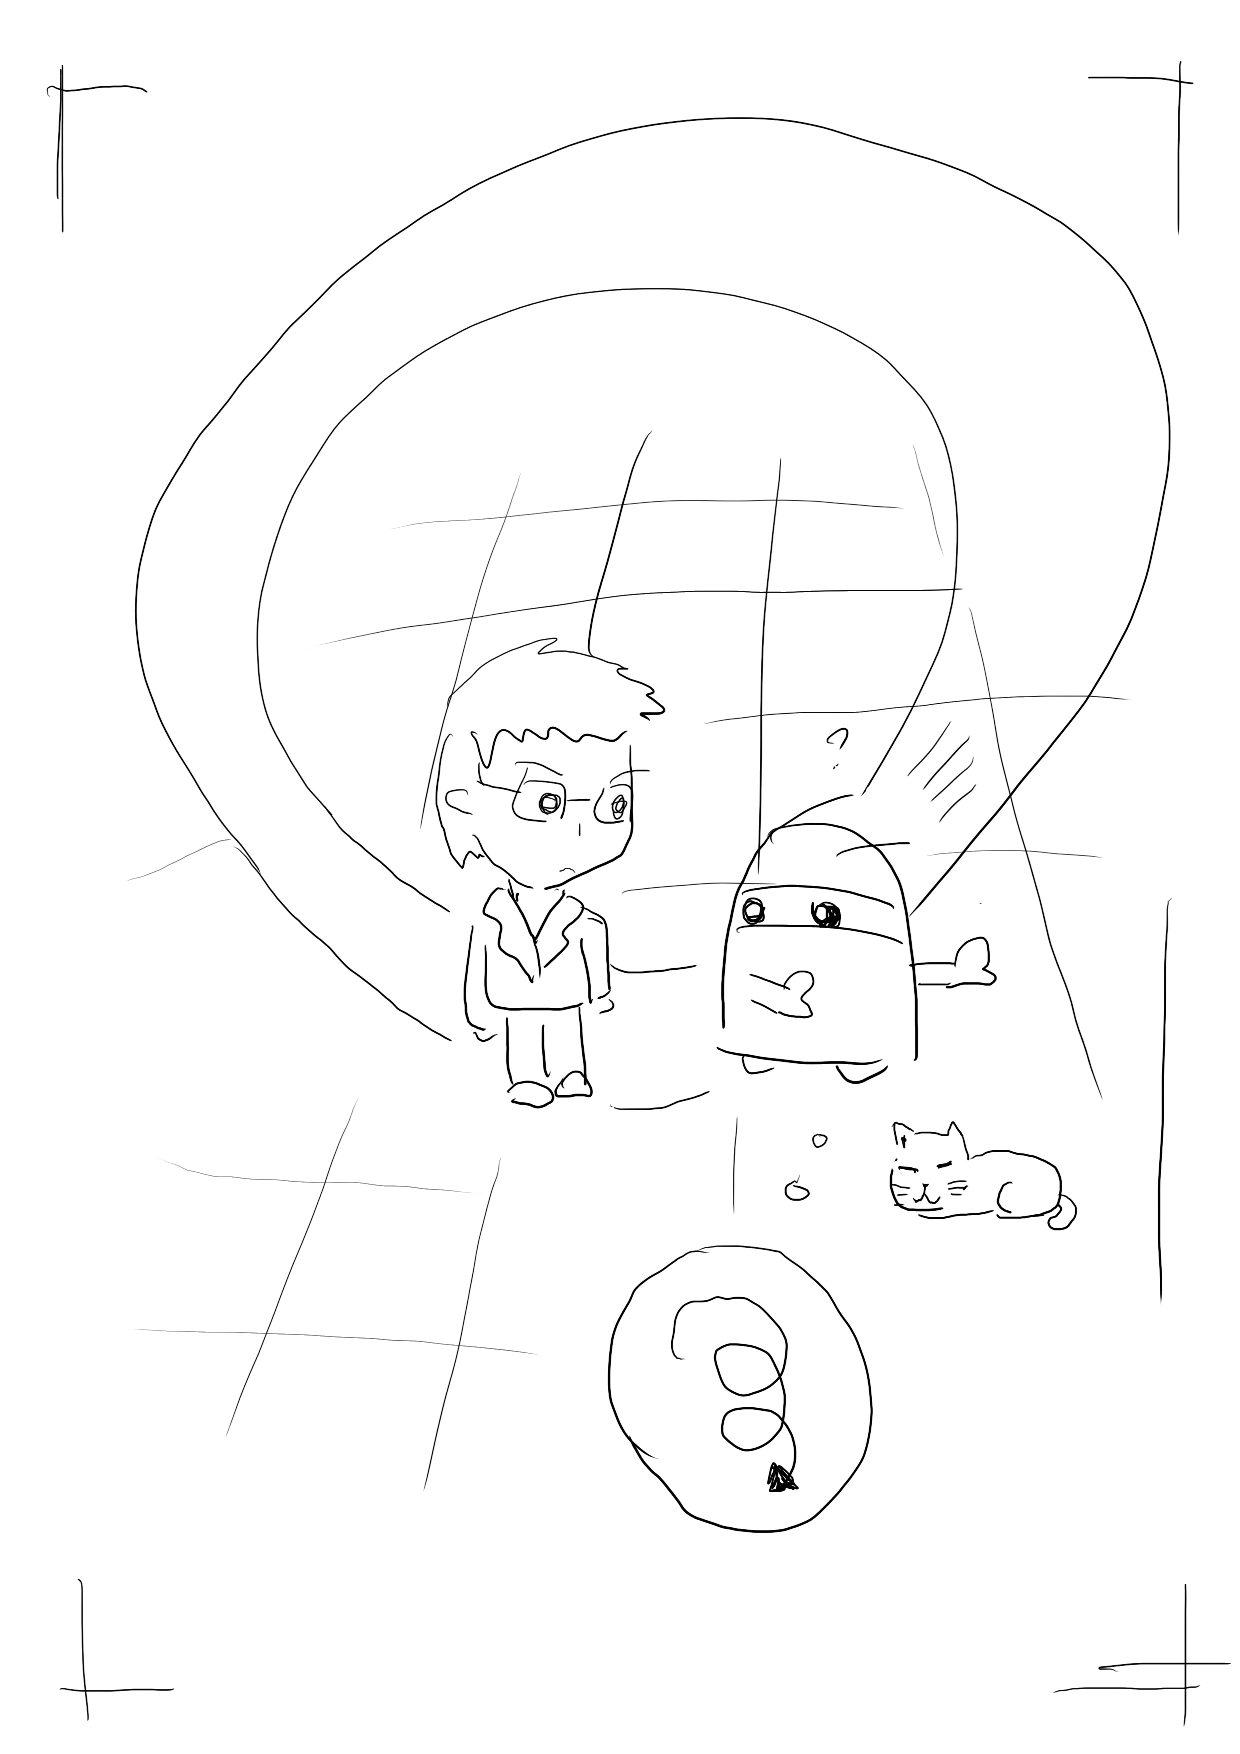
\includepdf{resources/other/ch12.pdf}

\newpage
\section{Loop Closure and Detection}
\subsection{Why Loop Closure is Needed}
We have already introduced the front-end and the back-end: the front-end provides short-time trajectory/landmarks estimation and the map's initial value. The back-end is responsible for optimizing all these data. However, if we only consider the adjacent keyframes like VO, then the errors will inevitably accumulate with time so that the entire SLAM will suffer from the accumulative error. The result of long-term estimation will not be reliable. In other words, we cannot construct \textbf{globally consistent} trajectories and maps.

Let's take an example. In the map-building stage of autonomous driving, we usually designate the collection vehicle to circle several times in a given area to cover all the collection areas. Suppose we extract the features at the front end, then ignore the feature points, and use a pose graph to optimize the entire trajectory at the back end, as shown in \autoref{fig:drift}(a)~. Since the frontend gives only partial pose constraints, for example, it may be $\bm{x}_1-\bm{x}_2, \bm{x}_2-\bm{x}_3$, etc. However, due to the error in the estimation of $\bm{x}_1$, $\bm{x}_2$ is determined according to $\bm{x}_1$, $\bm{x}_3$ is again determined by $ \bm{x}_2$. By analogy, errors will be accumulated, making the result of back-end optimization look like what is shown in \autoref{fig:drift}~(b), which gradually tends to be inaccurate. In this application scenario, we should use the loop closure information to determine that the vehicle reaches the same place when we pass the same road.

\begin{figure}[!htp]
	\centering
	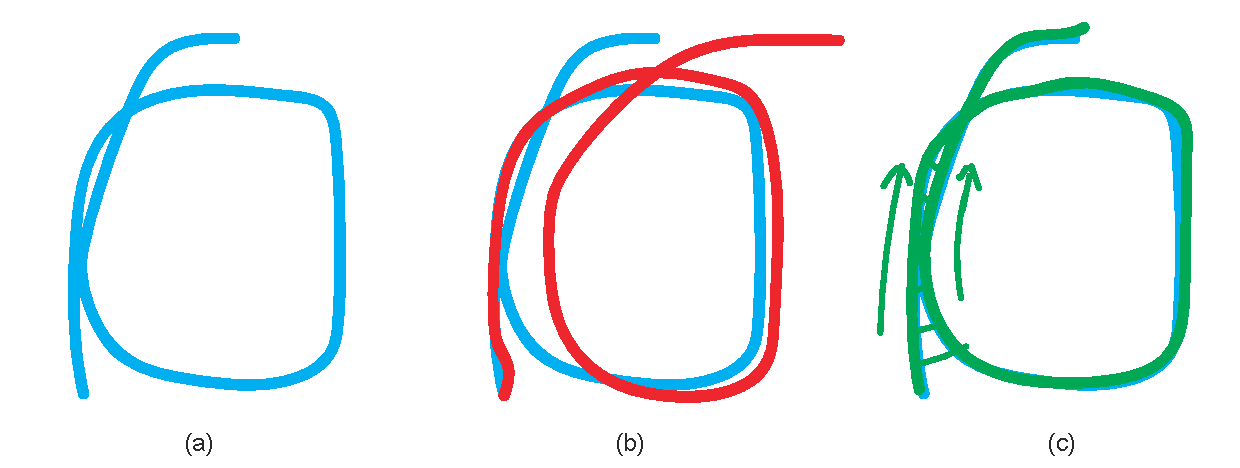
\includegraphics[width=0.8\textwidth]{loopclosure/illustrate-loop.pdf}
	\caption{Accumulated drift. (a) Real trajectory. (b) Accumulated error if we only consider adjacent keyframes. (c) Add loop closure to reduce the accumulated drift. }
	\label{fig:drift}
\end{figure}

Although the backend can estimate the maximum posterior error, it depends on the structure of the BA or the pose graph. If there are only adjacent keyframe constraints, we cannot do much, nor can we eliminate the accumulated error. However, the loop closure detection module can give some constraints on \textbf{longer time} other than adjacent frames: for example, the pose constraint between $\bm{x}_1-\bm{x}_{100}$. Why are there constraints between them? Because we noticed that the camera returns to a previously visited scene, and it acquires similar data ln history. The key to loop detection is how to detect this fact effectively. If we can successfully detect this, we can provide more valid constraints for the backend pose graph to get a better estimate, especially a globally consistent estimate. Since the pose graph can be regarded as a point-spring system, loop detection is equivalent to adding additional springs to the graph, which improves the system's stability. The reader can also intuitively imagine that the loop edge "pulls" the edge with accumulated error back to the correct position-if the loop itself is correct.

Loop detection is of great significance to SLAM systems. It is related to the correctness of our estimated trajectory and map in \textbf{long time}. On the other hand, since loop detection provides the correlation between current data and historical data, we can also use loop detection for \textbf{relocation}. Relocation is also beneficial in most applications. For example, if we record a track for a scene in advance and build a map, then we can let the robot follow this track for navigation, and relocation can help us determine our position on this track. Therefore, the loop detection improves the accuracy and robustness of the entire SLAM system. In some cases, we call a system with only a front-end and a local backend as \textbf{VO} and call a system with loop closing and a global backend as \textbf{SLAM}.

\subsection{How to Close the Loops}
Let's consider how to implement loop detection. There are several different ways of thinking about this problem, including theoretical and engineering.

The simplest way is to perform feature matching on any image pairs and determine which of them are related according to the number of correct matches. This is indeed a simple and effective idea. The disadvantage is that we blindly assume that "any two images may have loops," which makes the number of detection too large: for $N$ possible loops, we have to detect $C_N^2$ times. It has the complexity of $O(N^2)$, which grows too fast as the trajectory becomes longer and is not practical in most real-time systems. Another simple way is to extract historical data and perform loop detection randomly. For example, randomly select five frames among $n$ frames and compare them with the current frame. This approach can maintain a constant time calculation, but when the number of frames $N$ increases, the probability of drawing a loop is significantly reduced, making the detection efficiency low.

The simple ideas mentioned above are too coarse. Although random detection is indeed useful in some implementations like {\cite{Endres2014}}, we at least hope that there is a prediction of "there may be a loop somewhere" so that the detection is not so blind. Such approaches can be roughly divided into two ideas: odometry-based or appearance-based. Based on the geometric relationship, when we find that the current camera moves close to a certain position before, we detect whether they have a loop relationship \cite{Hahnel2003}. This is naturally an intuitive idea, but it is hard to estimate the accumulated drift amount unless we have global position measurements like GPS. Therefore, this approach has a logical problem because the goal of loop detection is to eliminate accumulated errors. But the odometry-based approach assumes that "the accumulated error is small so that the loop can be detected." If the assumption does not hold, such methods cannot work when the cumulative error is large \cite{Beeson2010}.

The other method is based on appearance. It has nothing to do with the estimation of the frontend or the backend and only determines the loop detection relationship based on the two images' similarity. This approach eliminates accumulated errors and makes the loop detection module a relatively independent module in the SLAM system (of course, the frontend can provide the extracted feature points). Since it was proposed in the early 21st century, the appearance-based loop detection method can effectively work in different scenarios and has become the mainstream method in visual SLAM and applied to the actual system {\cite{Ulrich2000, Latif2013, Mur-Artal2015}}.

In the appearance-based loop detection algorithm, the core problem is how to calculate the similarity between images. For example, for image $\bm{A}$ and image $\bm{B}$, we need to design a method to calculate the similarity score between them: $s(\bm{A}, \bm{B })$. Of course, this score will take a value in a certain interval, and when it is greater than a certain amount, we think that there is a loop. Readers may have questions: Is it difficult to calculate the similarity between two images? For example, intuitively, an image can be expressed as a matrix, so how about subtracting two images directly and then taking a certain norm?

\begin{equation}
	s(\bm{A}, \bm{B}) = \| \bm{A}-\bm{B} \|.
\end{equation}

Why don't we do this?

\begin{enumerate}
	\item As mentioned earlier, the pixel grayscale is an unstable measurement value, which is severely affected by the ambient light and camera exposure. Assuming that the camera is not moving and we turn on an electric light, the image will be brighter overall. In this way, even for the same data, we will get a significant difference value.
	\item On the other hand, when the camera's viewing angle changes a little, even if each object's luminosity does not change, their pixels will be transformed in the image, resulting in a large difference in value.
\end{enumerate}

Due to the existence of these two situations, in practice, even for very similar images, $\bm{A}-\bm{B}$ will often get an (unrealistic) enormous value. So we say that this function {cannot reflect the similar relationship between images}. It involves a definition of ``good'' and ``bad.'' We have to ask, what kind of function can better reflect the similar relationship, and what kind of function is not good enough? From here, two concepts can be drawn: \textbf{perceptual aliasing} and \textbf{perceptual variability}. Let's discuss it in more detail now.

\subsection{Precision and Recall}
From a human point of view (at least we think), we can feel the fact that "the two images are similar" or "the two photos were taken from the same place" with high accuracy. But since we have not yet grasped the human brain's working principle, we cannot clearly describe how we accomplish this. From a program point of view, we hope that algorithms can reach judgments consistent with humans or facts. When we feel that the two images were taken from the same place, we expect the loop detection algorithm to give the same result as "this is a loop." Conversely, if we think that the two images were taken from different places, then the program should also give a judgment that "this is not a loop." Readers with a machine learning background should feel how similar this passage is to machine learning.  Of course, the judgment of the algorithm is not always consistent with our human thinking, so there may be four situations in \autoref{table:loopclosure}~:


\begin{table}[!htp]
	\centering
	\caption{Classification of the loop detection results}
	\label{table:loopclosure}
	\begin{tabu}{c|c|c}
		\toprule
		Algorithm $\backslash$ Fact & Is loop & Not loop\\ 
		\midrule
		Is loop & True Positive & False Positive \\ 
		Not loop & False Negative & True Negative\\ 
		\bottomrule
	\end{tabu} 
\end{table}

The term negative/positive come from medical terms. False-positive is also called perceptual bias, and false negative is called perceptual variation (see \autoref{fig:FPandFN}). For the convenience of writing, we use the abbreviation TP for true-positive, and FN for false-negative, etc. Since we want the algorithm to be consistent with human judgment, we hope that TP and TN should be as high as possible, and FP and FN should be as low as possible. Therefore, for a particular algorithm, we can count the number of occurrences of TP, TN, FP, and FN on a certain data set, and calculate two statistics: \textbf{accuracy rate} and \textbf{recall rate} (precision \& recall)
\begin{equation}
	\mathrm{Precision} = \mathrm{TP}/(\mathrm{TP}+\mathrm{FP}), \quad \mathrm{Recall} = \mathrm{TP}/(\mathrm{TP}+\mathrm{FN}).
\end{equation}

\begin{figure}[!htp]
	\centering
	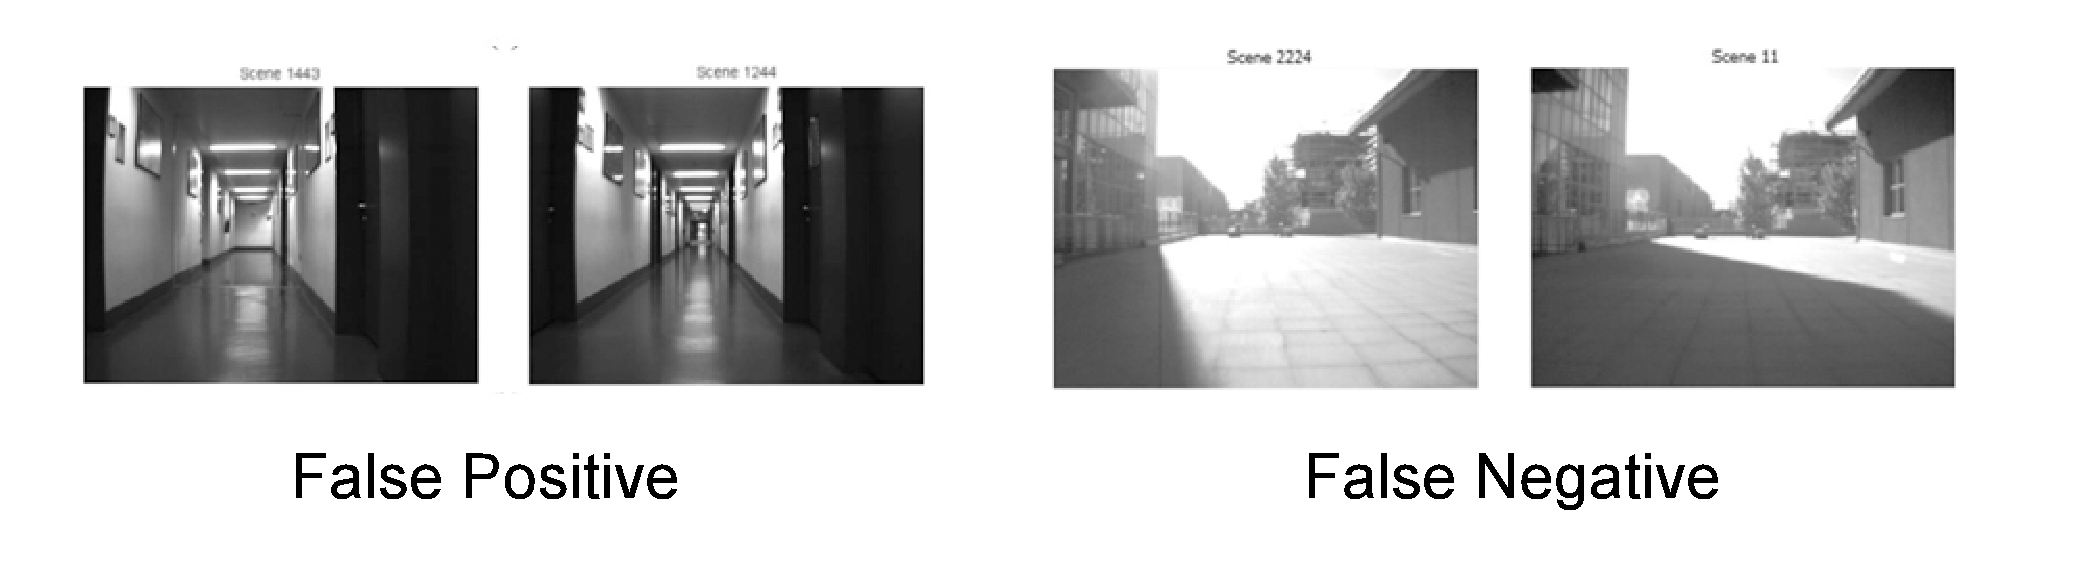
\includegraphics[width=0.9\textwidth]{loopclosure/FPandFN}
	\caption{Example of false-positive and false-negative scenes. Left: the images look same but actually taken from different space. Right: the images are from the same place but the appearance is different.}
	\label{fig:FPandFN}
\end{figure}

Literally, the accuracy rate describes the probability that all the loops extracted by the algorithm are indeed true loops. The recall rate refers to the probability of loops being detected from all real loops. Why shall we take these two statistics? Because they are representative and usually a pair of \textbf{contradiction}.

An algorithm often has many setting parameters. For example, when a certain threshold is raised, the algorithm may become more ``strict''. It detects fewer loops and improves accuracy. But at the same time, because the number of detection has decreased, many real loops may be missed, resulting in a decline in the recall rate. Conversely, if we choose a more relaxed configuration, the number of detected loops will increase, resulting in a higher recall rate. But there may be incorrectly detected loops so that the accuracy rate will decrease.

In order to evaluate the quality of the algorithm, we will test its $P$ and $R$ values under various configurations and then make a precision-recall curve (see \autoref{fig:PRCurve}). When using the recall rate on the horizontal axis and the accuracy rate on the vertical axis, we will care about the degree to which the entire curve deviates to the upper right, the recall rate at 100\% accuracy or the accuracy at 50\% recall rate, as evaluation indicators. However, please note that we usually cannot say that algorithm A is better than algorithm B in general. We may say that A has a good recall rate when the accuracy rate is high, while B can guarantee a good accuracy rate when the recall rate is 70\%, and so on.

\begin{figure}[!ht]
	\centering
	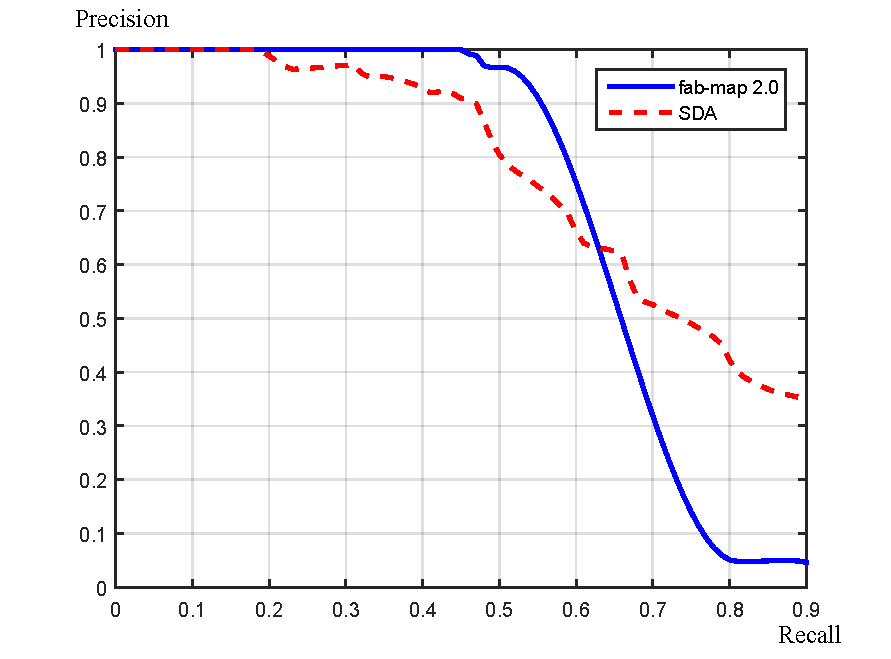
\includegraphics[width=0.66\textwidth]{loopclosure/prcurve}
	\caption{Example of the precision-recall curve {\cite{Gao2015a}}. As the recall rate increases, the detection conditions become looser and the accuracy rate decreases. A good algorithm can still guarantee a better accuracy rate in high recall rate.}
	\label{fig:PRCurve}
\end{figure}

It is worth mentioning that in SLAM, we have higher requirements for accuracy while being relatively tolerant to the recall. The false-positive loops will add fundamentally wrong edges to the backend pose graph, sometimes causing the optimization algorithm to give completely wrong results. Imagine if the SLAM mistakenly treats all the desks as the same one. What will happen to the created map? You may see that the corridor is not straight, the walls are staggered, and finally, the entire map is invalid. In contrast, if the recall rate is lower, some loops are probably not detected, and the map may be affected by some accumulated errors, but the other loops may eliminate them. Therefore, when choosing the loop detection algorithm, we are more inclined to set the parameters more strictly or add the step of \textbf{loop verification} after the detection.

So, back to the previous question, why not use $\bm{A}-\bm{B}$ to calculate similarity? We will find that its accuracy and recall are inferior to most current methods, and there may be many false-positive or false-negative cases, so it is ``not good.'' So, which method is better?

\section{Bag of Words}
Since directly subtracting two images is not good enough, then we need a more reliable method. Recalling the previous lectures' content, we may have an intuitive idea: Why not use feature points from VO to detect the loops? We may match the feature points of the two images just like VO. Furthermore, according to the feature matching, we can also calculate the motion between the two images. Of course, there are some problems with this approach. For example, feature matching will be time-consuming, feature description may be unstable when the illumination changes, etc., but it is very close to the bag of words model we are going to introduce. Let's talk about the bag of words first and then discuss the implementation details.

Bag-of-Words (BoW), the purpose is to describe an image in terms of "what kinds of features are there on the image." For example, we say that there are a person and a car in one photo; and two people and a dog in another photo. According to this description, the similarity of the two images can be measured. To be more specific, we need to do the following things:

\begin{enumerate}
	\item Determine the concepts of people, cars, and dogs-corresponding to the word. Many words are put together to form a dictionary.
	\item Detect which predefined words in the dictionary appear in an image-we use the appearance of words (histogram) to describe the entire image. In this way, we convert an image into a vector description.
	\item Compute the similarity by the histogram in the second step.
\end{enumerate}


Let's give an example. Assume we get a dictionary in some way. There are many words recorded in the dictionary, and each word has a certain meaning. For example, \textit{person}, \textit{car}, and \textit{dog} are all words recorded in the dictionary. We might as well write them as $w_1, w_2, w_3$. Then, for any image A, according to the words they contain, it can be written as:
\begin{equation}
	A = 1 \cdot w_1+1\cdot w_2 + 0 \cdot w_3.
\end{equation}

Since the dictionary is fixed, we may use the vector $[1,1,0]^\mathrm{T}$ to express the meaning of $A$. Through dictionaries and words, only one vector can describe the entire image. This vector describes the information of "whether the image contains a certain type of feature," which is more stable than pure gray value. And because the description vector is only about the existence of the words rather than their order, it has nothing to do with the object's spatial position and arrangement order. Therefore, when the camera moves a little, as long as the object is appearing in the field of vision, we still guarantee that the description vector does not change \footnote{Although this property sometimes brings some problems, for example, is the face with the eyes under the mouth still a human face? }. Based on this feature, we call it Bag-of-Words instead of List-of-Words. The emphasis is on the presence or absence of Words, regardless of their order. Therefore, it can be said that a dictionary is similar to a collection of words.

Going back to the above example, in the same way, the vector $[2,0,1]^\mathrm{T}$ can describe the image $B$. If you only consider "whether it appears" without considering the quantity, it can also be $[1,0,1]^\mathrm{T}$. At this time, this vector is binary. Therefore, by designing a certain calculation method based on these two vectors, the similarity between the images can be determined. Of course, if there are still some different ways to calculate the difference between two vectors, for example, for $\bm{a}, \bm{b} \in \mathbb{R}^W$, you can calculate:
\begin{equation}
	s\left( {\bm{a},\bm{b}} \right) = 1 - \frac{1}{W}\left\| {\bm{a} - \bm{b}} \right\|_1,
\end{equation}
where we take the $L_1$ norm, which is the sum of the absolute values of the elements. Please note that when the two vectors are exactly the same, we will get 1; when the two vectors are completely different (where $\bm{a}$ is 0, $\bm{b}$ is 1), we will get 0. This defines the similarity of the two description vectors, and also defines the degree of similarity between the images.

Yes, what's next?
\begin{enumerate}
	\item How does the dictionary come from?
	\item If we can calculate the similarity score between two images, is it enough to close the loop?
\end{enumerate}

Next, we first introduce the generation method of the dictionary and then introduce how to use the dictionary to calculate the similarity between two images.

\section{Train the Dictionary}
\subsection{The Structure of Dictionary}
According to the previous introduction, the dictionary is composed of many words, and each word represents a concept. A word is different from a single feature point. It is not extracted from a single image, but a combination of a certain type of feature. Therefore, the dictionary generation problem is similar to a \textbf{clustering} (Clustering) problem.

The clustering problem is particularly common in unsupervised machine learning, which lets the machine find the data structure by itself. Training BoW's dictionary is also one of them. First, suppose we have extracted feature points from many, let's say $N$, images. Now, we want to find a dictionary with $k$ words. Each word can be regarded as a collection of local adjacent feature points. We can solve this with the classic K-means (K-means) algorithm {\cite{Lloyd1982}}.

K-means is a straightforward and effective method. It is widely used in unsupervised learning, and we briefly introduce its principles below. Let's say there are $N$ data, and you want to classify them into $k$ categories, then using K-means to do it mainly includes the following steps:

\begin{mdframed}
	\begin{enumerate}
		\item Randomly select $k$ centers: $c_1, \cdots, c_k$.
		\item Compute the distance between each data sample to the cluster centers. Assign the closest cluster to this sample. 
		\item Re-compute the centers of the clusters. 
		\item If the centers converge, exit. Otherwise return to step 2. 
	\end{enumerate}
\end{mdframed}







